\documentclass{article}

\usepackage{graphicx}
\usepackage{subcaption}
\usepackage{amssymb}
\usepackage[utf8]{inputenc}
\usepackage[T1]{fontenc}
\usepackage{framed}
\usepackage{wrapfig}

\title{Reporte de Actividad 8 - Oscilador de Van der Pol}

\author{Diego Iván Moreno Campa}

\date{10 de Abril, 2018}

\begin{document}

\maketitle

\bigskip

\section{Introducción}

En esta práctica se expandió en el uso de Python para resolver ecuaciones diferenciales no-lineales utilizando el paquete ODEint de SciPy. Específicamente, resolveremos un sistema de ecuaciones diferenciales conocido como el oscilador de Van der Pol.

Originalmente el oscilador de Van der Pol fue descubierto por un ingeniero eléctrico y físico Balthasar Van der Pol mientras trabajaba para phillips. Van der Pol obtuvo oscilaciones, las que luego llamo oscilaciones de relajación y ahora son conocidas como un tipo de ciclo límite en circuitos eléctricos que emplean tubos de vacío.

La ecuación de Van der Pol tiene larga historia de uso en la biología y la física. Por ejemplo, en biología, Fitzhugh y Nagumo extendieron la ecuación a un camplo plano como un modelo de potenciales de acción en neuronas.
\section{Modelo de Van der Pol}

El modelo de Van der Pol es un oscilador no-conservativo con amortiguamiento no-lineal. Evoluciona con el tiempo de acuerdo a la ecuacion diferencial de segundo orden:
\[ \frac{d^2x}{dt^2}-\mu(1-x^2)\frac{dx}{dt}+x=0 \]

donde $x$ es la posición coordenada, la cual es una función del tiempo $t$, y $\mu$ es un parametro escalar indicando la no-linealidad y la fuerza de amortiguamiento.

Para probar que el sistema tiene un ciclo límite se utiliza el teorema de Liénard, aplicando la transformación $y=x-x^3/3-\dot{x}/\mu$ se puede escribir el oscilador de Van der Pol en su forma dos-dimensional:
\[ \dot{x} = \mu \left(x-\frac{1}{3}x^3-y \right) \]
\[ \dot{y} = \frac{1}{\mu}x \]

otra manera común de escribir el oscilador de forma dos-dimensional es:
\[ \dot{x} = y \]
\[ \dot{y} = \mu(1-x^2)y-x \]

De aquí tenemos dos características especiales cuando se tiene el oscilador no forzado.
Sí $\mu=0$ el oscilador se simplifica a la forma ya que no hay amortiguamiento:
\[ \frac{d^2x}{dt^2}+x=0 \]
Y cuando $\mu>0$ el sistema entra a un ciclo límite, mostrando inestabilidad cerca del origen mientras que es amortiguado lejos de este.



Si consideramos una fuerza oscilatoria actuando sobre el oscilador Van der Pol simplemente se toma la ecuación original y se agrega el forzamiento con la expresión $A\sin\omega t$:
\[ \frac{d^2x}{dt^2}-\mu(1-x^2)\frac{dx}{dt}+x-A\sin\omega t=0 \]
donde A es la magnitud de la oscilación y $\omega$ la velocidad angular de la oscilación.

\section{Soluciones del modelo en Espacio Fase}

Utilizando la forma bidimensional alternativa de la ecuación oscilatoria de Van der Pol
\[ \dot{x} = y \]
\[ \dot{y} = \mu(1-x^2)y-x \]
podemos escribirla fácilmente en Python para resolverla utilizando ODEint de SciPy:
~\\
\hrule
\begin{verbatim}
def vectorfield(w, t, mu):
    
    x, y = w

    # Create f = (x',y'):
    f = [y,
         mu*(1.0 - x**2.0) * y - x]
    return f

\end{verbatim}
\hrule
~\\
donde $x$ y $y$ son variables y $mu$ es un parametro.

\newpage

Para obtener las soluciones en el espacio fase requerimos crear archivos con listas de datos como las prácticas anteriores con el código:

~\\
\hrule
\begin{verbatim}
# Parameter values
# Damping coefficient:
mu = 2.0
# Initial conditions
# x is the initial displacement and y is the initial velocity
x = -3.0
y = -3.0

stoptime = 50.0
numpoints = 2500
t = [stoptime * float(i) / (numpoints - 1) for i in range(numpoints)]

# Pack up the parameters and initial conditions:
w0 = [x, y]

# Call the ODE solver.
wsol = odeint(vectorfield, w0, t, args=(mu,))

with open('act8-a.dat', 'w') as f:
    # Print & save the solution.
    for t1, w1 in zip(t, wsol):
        print (t1, w1[0], w1[1], file=f)
\end{verbatim}
\hrule 
~\\

De esta manera tenemos un listado de datos con condiciones iniciales $x(0)=-3.0$ y $\dot{x}(0)=-3.0$ y parametro no-lineal $\mu=2.0$ de la que se obtiene la siguiente gráfica:
\begin{figure}[ht!]
\centering
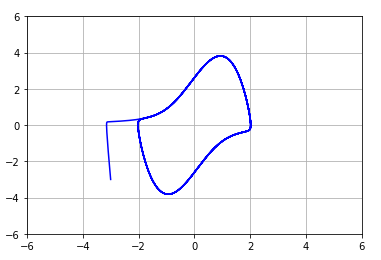
\includegraphics[width=0.5\linewidth]{act8a.png}
\caption{Retrato de fase para una solución de condiciones iniciales$x(0)=-3.0,\dot{x}(0)=-3.0$}
\end{figure}

\newpage

De la figura 1 se puede notar que la solución converge a un ciclo límite, esto ocurre para cualquier pareja de condiciones iniciales. Si nosotros gráficamos varias soluciones en un plano podemos observar las distintas soluciones convergiendo al ciclo límite marcado en rojo:

\begin{figure}[ht!]
\centering
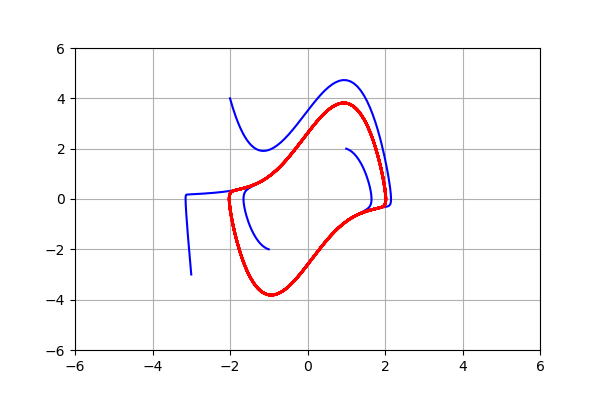
\includegraphics[width=0.5\linewidth]{fig2.png}
\caption{Retrato de fase para varias soluciones que convergen a un ciclo limite con parametro no-lineal $\mu=2.0$}
\end{figure}

Obtuvimos el ciclo límite para $\mu=2.0$ y al simplemente ajustar este parametro se pueden obtener diferentes ciclos límite como se muestra en la figura 3 a continuación.
\begin{figure}[ht!]
\centering
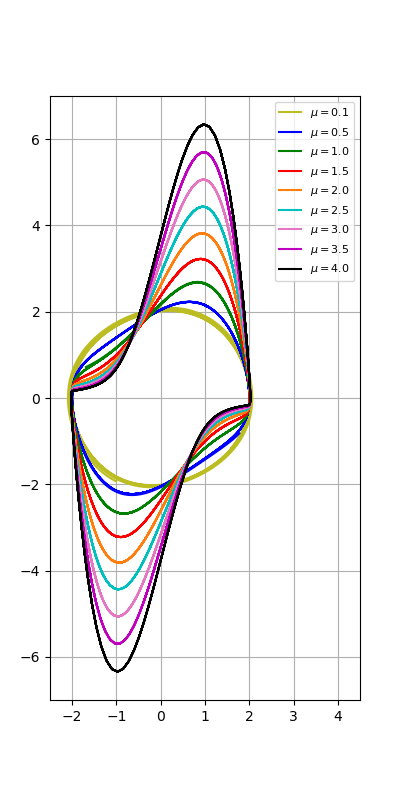
\includegraphics[width=0.42\linewidth]{fig3.png}
\caption{Ciclos límite para distintos valores de $\mu$}
\end{figure}

\newpage

Para obtener la gráfica anterior generamos varios listados de archivo con cualesquiera condiciones iniciales pero con distintos valores de $\mu$ que van desde $0.1$ a $4.0$, después los gráficamos en el mismo plano:

~\\
\hrule
\begin{verbatim}
import matplotlib as mpl
%matplotlib inline

figure(figsize=(4, 8))

t, x, y = loadtxt('act8-0.dat', unpack=True, skiprows=1000)
plot(x,y,'tab:olive')

t, x, y = loadtxt('act8-1.dat', unpack=True, skiprows=300)
plot(x,y,'b')

t, x, y = loadtxt('act8-2.dat', unpack=True, skiprows=150)
plot(x,y,'g')

t, x, y = loadtxt('act8-3.dat', unpack=True, skiprows=150)
plot(x,y,'r')

t, x, y = loadtxt('act8-4.dat', unpack=True, skiprows=150)
plot(x,y,'tab:orange')

t, x, y = loadtxt('act8-5.dat', unpack=True, skiprows=150)
plot(x,y,'c')

t, x, y = loadtxt('act8-6.dat', unpack=True, skiprows=150)
plot(x,y,'tab:pink')

t, x, y = loadtxt('act8-7.dat', unpack=True, skiprows=150)
plot(x,y,'m')

t, x, y = loadtxt('act8-8.dat', unpack=True, skiprows=150)
plot(x,y,'k')

legend((r'$\mu=0.1$',r'$\mu=0.5$', r'$\mu=1.0$',r'$\mu=1.5$',r'$\mu=2.0$',r'$\mu=2.5$',
r'$\mu=3.0$',r'$\mu=3.5$',r'$\mu=4.0$'), prop=FontProperties(size=8))

xlim(-2.5,4.5)
ylim(-7,7)
grid(True)
mpl.pyplot.axis('on')
savefig('fig3.png', dpi=100)
\end{verbatim}
\hrule 
~\\

Con el mismo método con el que gráficamos las soluciones en el espacio fase, podemos observar las oscilaciones que se presentan al gráficar la posición con respecto al tiempo:

~\\
\hrule
\begin{verbatim}
from numpy import loadtxt
from pylab import figure, plot, ylabel, xlabel, grid, hold, legend
	, title, savefig, ylim, xlim
from matplotlib.font_manager import FontProperties
%matplotlib inline

t, x, y = loadtxt('act8-relax.dat', unpack=True)

figure(1, figsize=(12, 2))

ylabel('$x_1$')
xlabel('t')
grid(True)
#hold(True)
lw = 2

ylim(-4, 4)
xlim(10,50)

plot(t, x, 'b', linewidth=lw)

savefig('fig1.png', dpi=100)
\end{verbatim}
\hrule
~\\

con lo que tenemos la siguiente gráfica:
\begin{figure}[ht!]
\centering
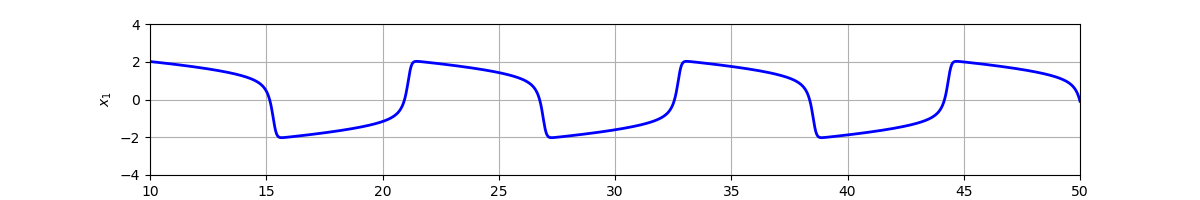
\includegraphics[width=\linewidth]{fig1.png}
\caption{Oscilaciones amortiguadas sin forzamiento con $\mu=5.0$}
\end{figure}

\newpage

En contraste, si deseamos estudiar el movimiento del oscilador forzado, agregamos a la ecuacion que describe nuestro sistema un término que describa una función impulsora $A\sin\omega t$ donde A es la amplitud y $\omega$ es la frecuencia de oscilación:

~\\
\hrule
\begin{verbatim}
import numpy as np
def forced(w, t, p):
    
    x, y = w
    
    A, om, mu = p

    # Create f = (x',y'):
    f = [y,
         mu*(1.0 - x**2.0) * y - x + A*np.sin(om*t)]
    return f
\end{verbatim}
\hrule
~\\

obtenemos la siguiente gráfica:
\begin{figure}[ht!]
\centering
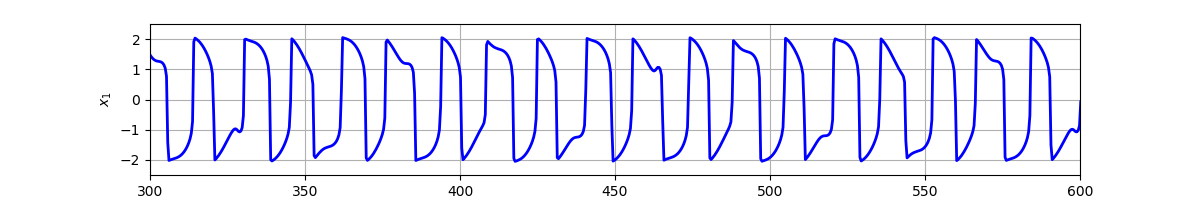
\includegraphics[width=\linewidth]{fig4.png}
\caption{Oscilaciones amortiguadas con forzamiento con parametros $\mu=8.53$, $A=1.2$ y $\omega=\frac{2\pi}{10}$}
\end{figure}

\section{Resultados}

En esta práctica obtuvimos varias gráficas que nos cuentan cosas distintas sobre el comportamiento del oscilador de Van der Pol.
En la Figura 1 podemos ver el cíclo limite marcado en rojo, sin importar las condiciones iniciales se llega al mismo atractor o ciclo límite. También notamos que el recorrido para llegar al ciclo límite es algo corto.

En la Figura 2 vemos que el atractor del oscilador depende del tamaño del coeficiente de no-linealidad, la forma del ciclo límite comienza como un circulo en valores de $\mu$ cercanos a cero hasta afilarse al incrementar $\mu$

Luego, en la figura 3 podemos observar las oscilaciones periódicas del oscilador de Van der Pol al tener ausencia de forzamiento, y por el contrario, notamos que en la figura 4 obtenemos oscilaciones caóticas al añadir el término de forzamiento.

\section{Conclusión}

En esta práctica podemos notar que es bastante fácil resolver simples ecuaciones diferenciales utilizando el mismo método de la práctica pasada, y que tambien hay varias opciones al gráficar soluciones para poder interpretar los resultados, como lo es visualizar el campo vectorial.

El oscilador de Van der Pol parece ser un oscilador bastante simple e interesante por el hecho de que fue descubierto al investigar para la compañia Phillips. Después de haber leído podemos ver que esta ecuación diferencial tiene varias aplicaciones interesantes, como la expansión que se realizó en ella para estudiar sistemas neuronales en biología.

\newpage

\section{Bibliografía}
\begin{itemize}
\item https://en.wikipedia.org/wiki/Van\_der\_Pol\_oscillator
\item http://www.scholarpedia.org/article/Van\_der\_Pol\_oscillator
\end{itemize}

\newpage

\title{Apéndice}

\begin{enumerate}
\item \textbf{Este ejercicio pareciera similar al desarrollado en las actividades 6 y 7. ¿Qué aprendiste nuevo?} ~\\~\\

Creo que no aprendí nada nuevo, solo me sirvió bastante para reforzar mi conocimiento de las práctica pasadas.

\item \textbf{¿Qué fue lo que más te llamó la atención del oscilador de Van der Pol? }~\\~\\

sus utilidades y el hecho de que fue descubierto mientras Balthasar trabajaba para Phillips el siglo pasado.

\item \textbf{Has escuchado ya hablar de caos. ¿Por qué sería importante estudiar este oscilador?}~\\~\\

para estudiar los patrones que emergen del caos para predecir parcialmente la evolución de un sistema y utilizar estos en nuestro favor

\item \textbf{¿Qué mejorarías en esta actividad?}~\\~\\
Nada, estuvo bien

\item \textbf{¿Algún comentario adicional antes de dejar de trabajar en Jupyter con Python?}  ~\\~\\
Dejar de trabajar en Jupyter con Python?!?!?!?!?!????


\item \textbf{Cerramos la parte de trabajo con Python ¿Que te ha parecido?} ~\\
Quisiera que estudiaramos más en Python, o si estudiamos resolución de sistemas de ecuaciones diferenciales en fortran no me molestaria o algun otro lenguaje.

\end{enumerate}

\end{document}
